\documentclass{article}
\usepackage{style-notes}

\newcounter{lecnum} 	% define counter for lecture number
\renewcommand{\thepage}{\thelecnum-\arabic{page}}	% define how page number is displayed (< lecture number > - < page number >)
% define lecture header and page numbers
% NOTE: to call use \lecture{< Lecture # >, < Lecture name >, < Chapter # >, < Chapter name >, < Section #s >}
\newcommand{\lecture}[5]{

    % define headers for first page
    \thispagestyle{empty} % removes page number from page where call is made

    \setcounter{lecnum}{#1}		% set lecture counter to argument specified

    % define header box
    \begin{center}
    \framebox{
      \vbox{\vspace{2mm}
    \hbox to 6.28in {\textbf{MATH 320: Probability} \hfill}
       \vspace{4mm}
       \hbox to 6.28in {{\hfill \Large{Lecture #1: #2} \hfill}}
       \vspace{2mm}
       \hbox to 6.28in {\hfill Chapter #3: #4 \small{(#5)}}
      \vspace{2mm}}
    }
    \end{center}
    \vspace{4mm}
    
    % define headers for subsequent pages
    \fancyhead[LE]{\textit{#2} \hfill \thepage} 		% set left header for even pages
    \fancyhead[RO]{\hfill \thepage}		% set right header for odd pages

}

% define macros (/shortcuts)
\newcommand{\bu}[1]{\textbf{\ul{#1}}}				% shortcut bold and underline text in one command
\newcommand{\blankul}[1]{\rule[-1.5mm]{#1}{0.15mm}}	% shortcut for blank underline, where the only option needed to specify is length (# and units (cm or mm, etc.)))
\newcommand{\comp}{{\sim}}						% shortcut for tilde without extra space, using for complement
\newcommand{\vecn}[2]{#1_1, \ldots, #1_{#2}}		% define vector (without parentheses, so when writing out in like a definition) of the form X_1, ..., X_n, where X and n are variable. NOTE: to call use $\vecn{X}{n}$


% NOTES on what didn't cover


\begin{document}

\lecture{6}{Bayes' Theorem}{1}{Probability}{1.5}

\bu{Law of total probability}\bigskip

Motivation\bigskip
\begin{itemize}
    \item Example: A company has three assembly lines. The first line, the second line and the third produce 30\%, 50\% and 20\% of productions, respectively.
    \item[] Additionally, 1 of 100 productions is defective in Line 1; 2 of 100 productions are defective in Line 2; 3 of 100 productions are defective in Line 3.
    \item[] We want to know the probability of defectives produced in the company.\smallskip
    \item \textit{STRATEGY}:
    \begin{enumerate}[(a)]
        \item Define all (unconditional) events given in the problem and find their probabilities. 
        \item[] If conditional events are given, define them using unconditional events.\vspace{60pt}
        \item Find the event of interest. Try to express the event of interest as a composition (union) of the given events.
        \item[] Often it is desirable to form compositions mutually exclusive or independent events.\vspace{30pt}
        \item Use the general multiplication rule to find the probability for the event of interest.\vspace{60pt}
    \end{enumerate}
    \item Visualizing scenario:
    \item[] (a) Using a Venn Diagram: \hspace{100pt} (b) Using a Tree Diagram:\vspace{100pt}
\end{itemize}\bigskip

Law of total probability\bigskip
\begin{itemize}
     \item The \textbf{law of total probability} says that a partition ($\vecn{A}{n}$) of the sample space will lead to a partition of any event $B$ into mutually exclusive pieces.\vspace{45pt}
    \item[] Then we can write $P(B)$ as the sum of the probabilities of those pieces. Note that an event $A$ and its complement $\comp{A}$ always partition $S$.
    \item Definition: \textbf{Law of total probability}
    \item[] Let $B$ be an event. If $\vecn{A}{n}$ partition the sample space, then\bigskip
    \item[] $P(B) =$ \vspace{85pt}
    \item Using the general tree diagram below, we can summarize
    \item[] Law of total probability = $P(\text{Second stage event}) = \sum \, \text{Branches of interest}$
    \begin{figure}[H]
        \center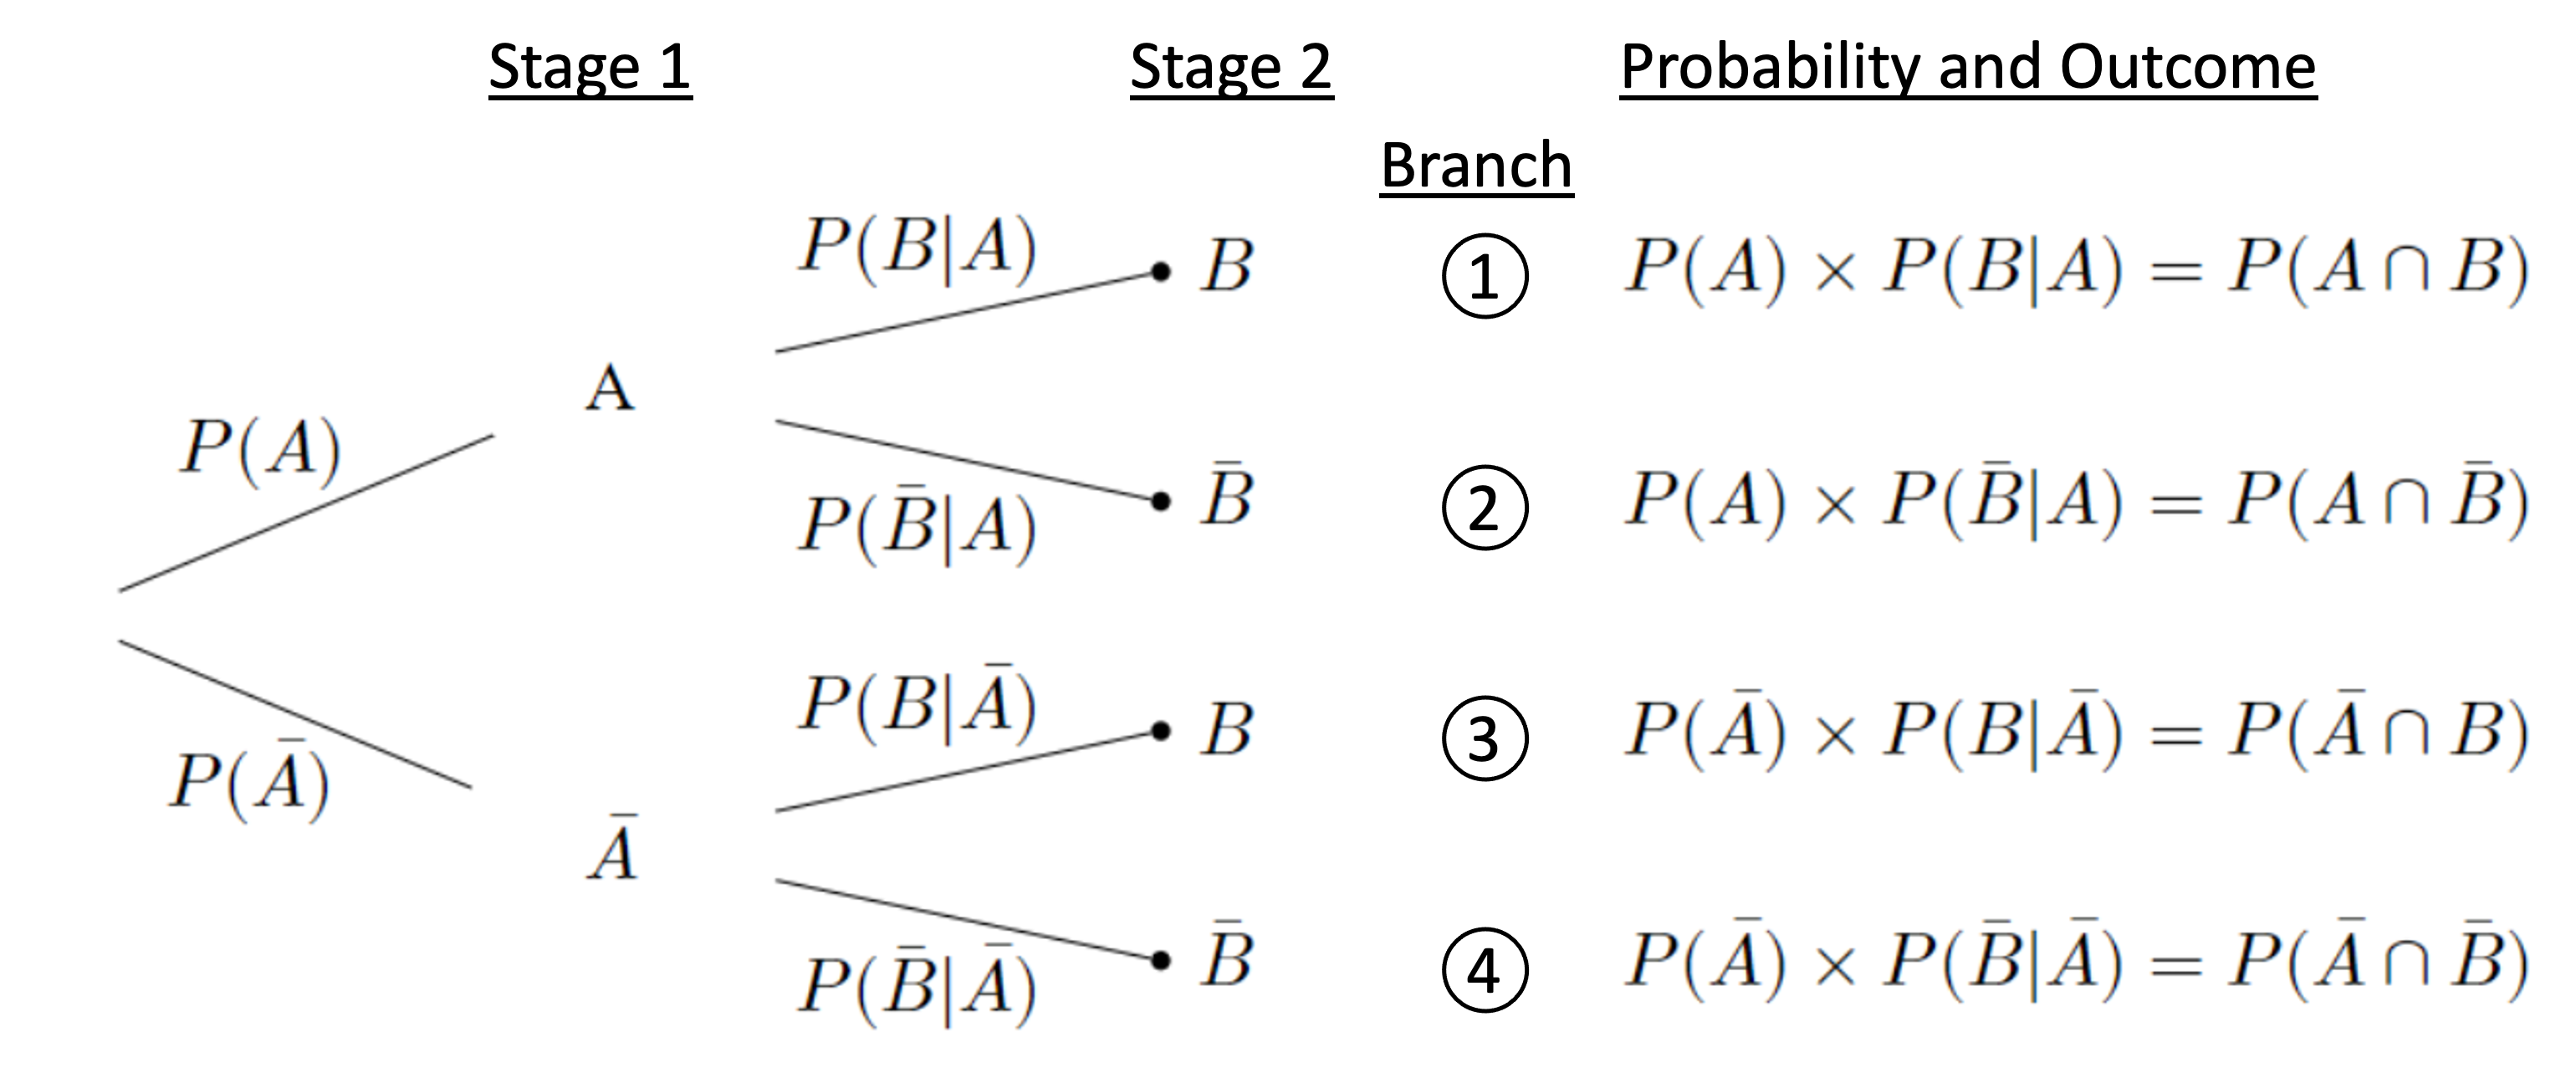
\includegraphics[scale=0.4]{test-1/general-tree-2}
    \end{figure}
\end{itemize}

\bu{Bayes' Theorem}\bigskip

Bayes' Theorem\bigskip
\begin{itemize}
    \item Using the same terminology, we can summarize
    \item[] Bayes' Theorem = $ P(\text{First stage event} \mid \text{Second stage event}) = \frac{\text{Main branch of interest}}{\sum \, \text{All branches of interest}}$
    \item In essence, Bayes' Theorem reverses the natural order of the tree for the conditional probability of interest.
    \item Continuing example:
    \item[] Find the probability that a defective product was made in Line 1.\vspace{100pt}
    \item Definition: \textbf{Bayes' Theorem}
    \item[] Let $B$ be an event. If $\vecn{A}{n}$ partition the sample space, then\bigskip
    \item[] $P(A_i \mid B) =$\vspace{50pt}
    \item Example: At the beginning of a certain study of a group of persons, 15\% were classified as heavy smokers, 30\% as light smokers, and 55\% as nonsmokers. In the five year study, it was determined that the death rates of the heavy and light smokers were five and three times that of the nonsmokers, respectively.
    \item[] A randomly selected participant died over the five-year period; calculate the probability that the participant was a nonsmoker.\vspace{100pt}
\end{itemize}\bigskip

Bayes' Theorem from another perspective\bigskip
\begin{itemize}
    \item Bayes' Theorem is all about changing probabilities based on new evidence.
    \item In a previous example, we drew a tree diagram about testing for the presence of a disease and the result of the test. We used the following events:
    \begin{flalign*}
       D &= \text{the person tested has the disease}&\\
       \comp D &= \text{the person tested does not have the disease}&\\
        Y &= \text{the test is positive}&\\
        N &= \text{the test is negative}&
     \end{flalign*}
     \item[] Lets now consider a disease test that is ``95\% accurate'', which can be defined as follows:
     \begin{enumerate}[a.]
         \item If you have the disease, 95\% chance of a positive test.
         \item If you do not have the disease, 95\% chance of a negative test.
     \end{enumerate}
    \item[] Further, suppose only 1\% of the population actually have this disease (aka prevalence).
     \begin{figure}[H]
         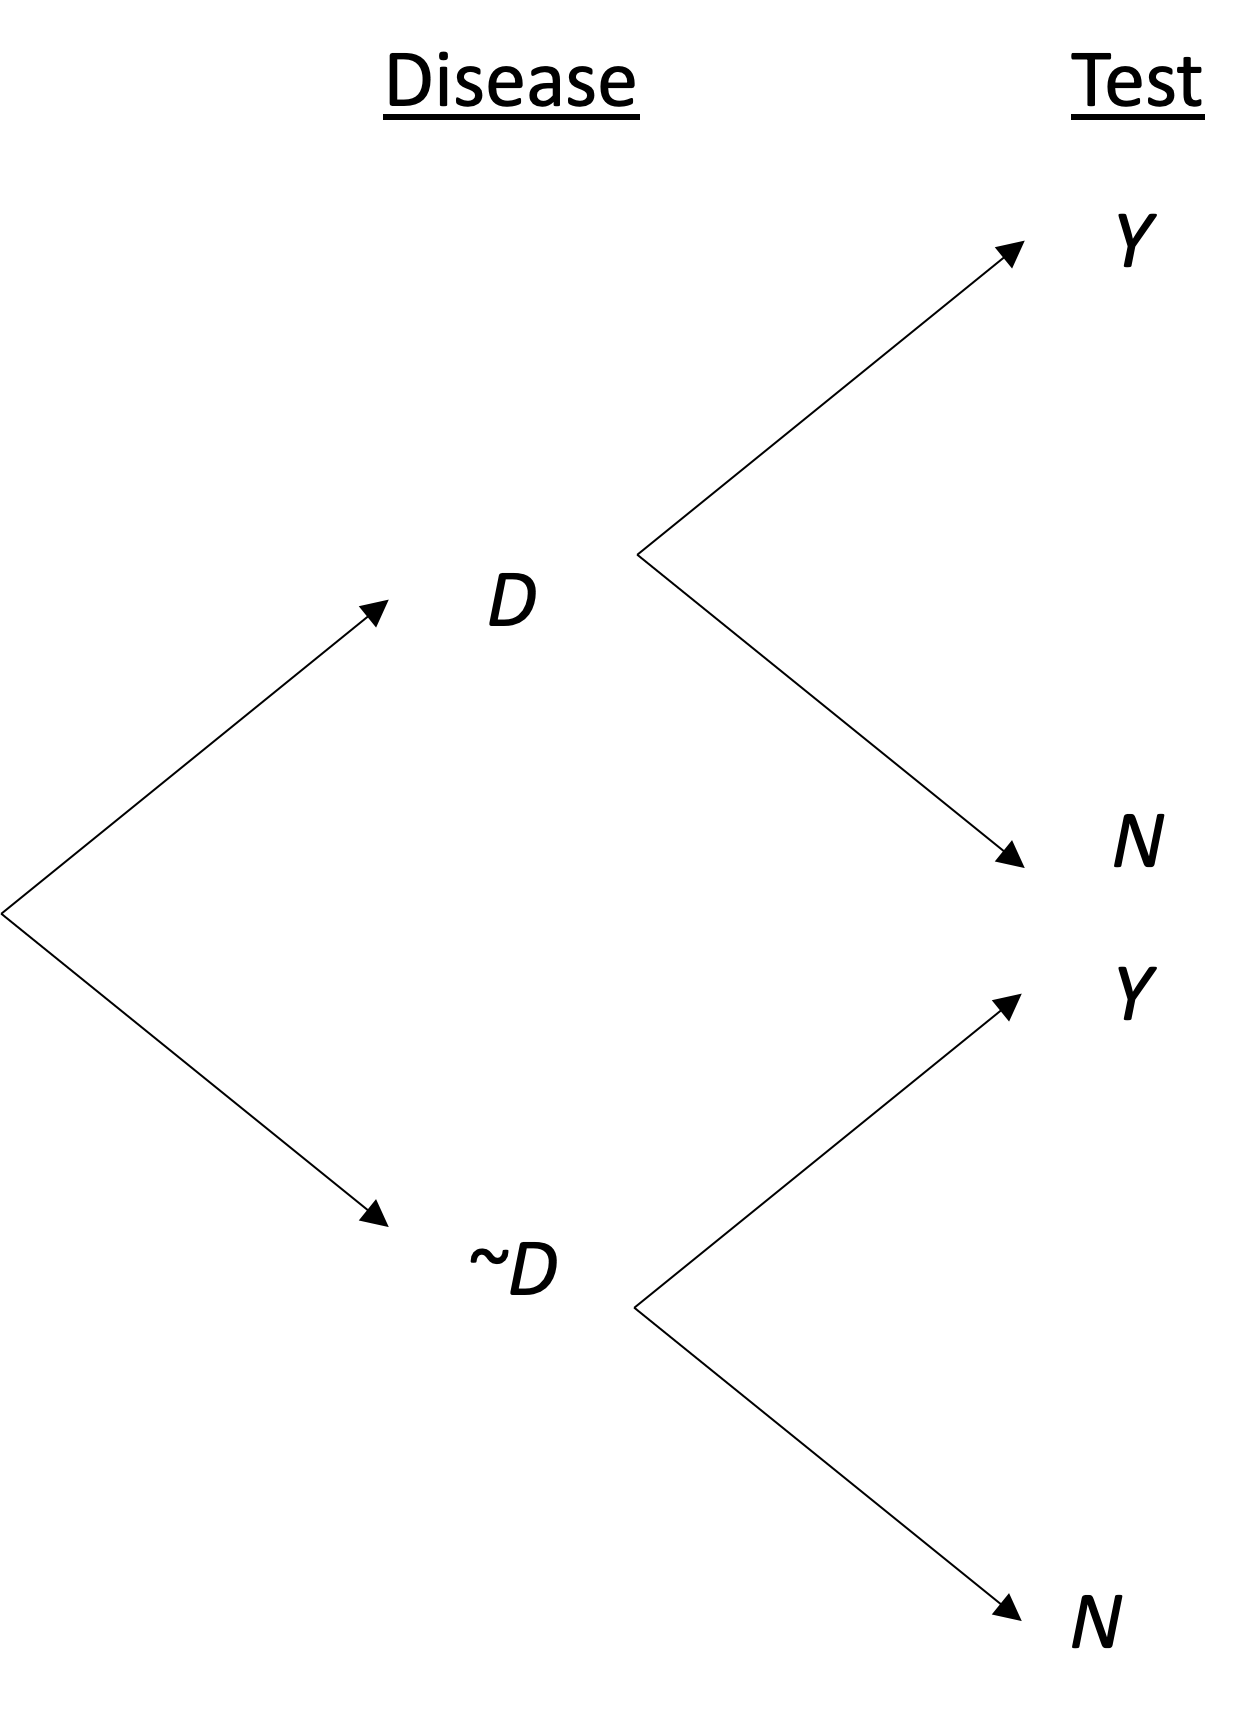
\includegraphics[scale=0.4]{test-1/tree-test}
     \end{figure}
     \item Terminology:
     \begin{itemize}
         \item Prior probability: Original unconditional probabilities
         \item Evidence: Conditional probability given the prior information
         \item Posterior probability: Prior probability conditioned on the new evidence
     \end{itemize}\bigskip
     \item Some calculations in context: The good and the bad of Bayes' Theorem
     \begin{enumerate}
         \item Find the probability of testing positive (total probability).\vspace{60pt}
         \item Lets' solve for the probability of having the disease \textit{given that you test positive}.
        \begin{enumerate}
            \item For a randomly selected person from the population, we had our original prior probability of having the disease, $P(D) = 0.01$.
            \item[] (We don't know if they do or don't have the disease, it remains unknown).\smallskip
            \item Then this person got tested, and tested positive; this is our evidence.\smallskip
            \item[] Intuitively, this likelihood of the person having the disease should \blankul{2cm}; we are adjusting the prior probability \blankul{2cm} based on the new evidence.\smallskip
            \item Now we can calculate this new posterior probability.\vspace{100pt}
        \end{enumerate}
        \item Suppose you know that someone has tested positive for this disease. What is the probability that the person does not actually have the disease?\vspace{90pt}
     \end{enumerate}
     \item The practical information here is interesting.
    \begin{enumerate}
        \item The "95\% accurate" test will classify \blankul{1cm} of the population as positives, compared to the true prevalence of $P(D) = 0.01$.
        \item By updating our prior probability with the new evidence, we drastically increased our information about this person having the disease. This is the good side of Bayes' Theorem! \vspace{20pt}
        \item \blankul{1cm} of the individuals who tested positive will actually \blankul{1cm} have the disease.
        \item[] This percentage depends heavily on the prevalence, for example if \\$P(D) = 0.1$ $\rightarrow$ $P(\comp{D} \mid Y) = $ \blankul{1cm}; and if $P(D) = 0.001$ $\rightarrow$ $P(\comp{D} \mid Y) = $\blankul{1cm}.
    \end{enumerate}
\end{itemize}\bigskip

Final example\bigskip
\begin{itemize}
    \item Alice writes to Bob and does not receive an answer. Assuming that one letter in $n$ is lost in the mail, find the probability that Bob received the letter. It is to be assumed that Bob would have answered the letter if he had received it.
    \item[] Let $A = $ Alice receives letter from Bob and $B = $ Bob receives letter from Alice.\vspace{100pt}
\end{itemize}








\end{document}